\documentclass{beamer}

\mode<presentation> {
\usetheme[secheader]{Madrid}
\usecolortheme{seahorse}
\useinnertheme{circles}
}

\usepackage{graphicx} % Allows including images
\usepackage{booktabs} % Allows the use of \toprule, \midrule and \bottomrule in tables
\usepackage{tikz}
\usepackage{url}

\setbeamerfont{section in sidebar}{size=\fontsize{5}{6}\selectfont}
\setbeamerfont{subsection in sidebar}{size=\fontsize{4}{5}\selectfont}
\setbeamerfont{subsubsection in sidebar}{size=\fontsize{3}{3}\selectfont}

%----------------------------------------------------------------------------------------
%	TITLE PAGE
%----------------------------------------------------------------------------------------

\title[Interaction Elements]{Interaction Elements} % The short title appears at the bottom of every slide, the full title is only on the title page

\author{Chaklam Silpasuwanchai} % Your name
\institute[AIT] % Your institution as it will appear on the bottom of every slide, may be shorthand to save space
{
Asian Institute of Technology \\ % Your institution for the title page
\medskip
\textit{chaklam@ait.asia} % Your email address
}
\date{} % Date, can be changed to a custom date

\AtBeginSection[]
{
\begin{frame}<beamer> 
\tableofcontents[currentsection]  % show TOC and highlight current section
\end{frame}
}

\begin{document}

\begin{frame}
\titlepage % Print the title page as the first slide
\end{frame}

\begin{frame}
\frametitle{Overview} % Table of contents slide, comment this block out to remove it
\tableofcontents % Throughout your presentation, if you choose to use \section{} and \subsection{} commands, these will automatically be printed on this slide as an overview of your presentation
\end{frame}

%----------------------------------------------------------------------------------------
%	PRESENTATION SLIDES
%----------------------------------------------------------------------------------------

%------------------------------------------------

\begin{frame}
\frametitle{Sources} 
\begin{itemize}
	\item Mackenzie, Chapter 3, \textbf{Interaction Elements},  Human Computer Interaction: An Empirical Research Perspective, 1st ed. (2013) 
\end{itemize}
\end{frame}

\section{Control-display relationships}

\begin{frame}
	\frametitle{Control-display relationships}
	\begin{itemize}
		\item \textbf{Control-display relationships} describe the mappings between \textbf{control} and \textbf{display}
		\item The mouse/cursor example describes a \textbf{spatial} relationship. There are also \textbf{dynamic} relationships, describing how a controller affects the speed of the response, and \textbf{physical} relationships, describing whether the response is to a movement or a force in the controller
	\end{itemize}
\end{frame}

\subsection{Spatial relationships}

\begin{frame}
	\frametitle{Spatial relationships}
	\begin{itemize}
		\item The mapping is \textbf{congruent} in left figure, while in right figure, you move the mouse forward which indicates up (fortunately, human can learn this relationship quite naturally)
	\end{itemize}
	\begin{figure}
		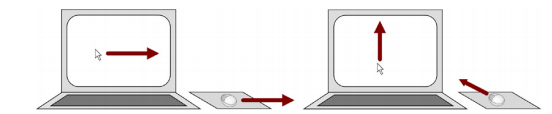
\includegraphics[width=1\linewidth]{image/3-4}
		\caption{Source: Figure 3.4 (Mackenzie)}
	\end{figure}
\end{frame}

\begin{frame}
	\footnotesize
	\frametitle{Definitions}
	\begin{itemize}
		\item \textbf{Control space} (a) depicts the possible movement of the input device
		\item \textbf{Display space} (b) depicts the corresponding display (e.g., cursor) movements
		\item \textbf{Control-display mappings} for a mouse and cursor (c) 
		\item The y-axis cursor motion is an example of a \textbf{transformed spatial mapping}.  In this case, it is a 90 deg transformation along the y-z plane
	\end{itemize}
	\begin{figure}
		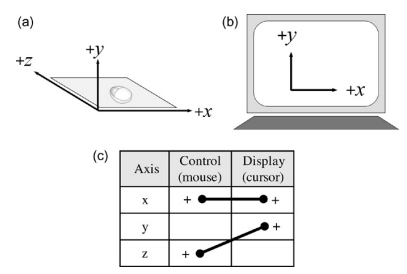
\includegraphics[width=0.5\linewidth]{image/3-5}
		\caption{Source: Figure 3.5 (Mackenzie)}
	\end{figure}
\end{frame}

%\begin{frame}
%	\frametitle{Performance}
%	\begin{itemize}
%		\item Effect of performance in the presence of a spatial transformation is well documented
%		\item \textbf{Aiming error} is known to be higher for 90 to 135 deg, and lower for 0 deg or 180 deg (Cunningham, 1989)
%		\item \textbf{Adaptations} take as few as 50 trials (Wigdor et al., 2006) - implying that humans are quite good at learning such transformation (in a subconscious manner)
%	\end{itemize}
%\end{frame}

\begin{frame}
	\frametitle{Scrolling}
	\begin{itemize}
		\item Consider \textbf{scrolling} the view of an image or document. Interaction involves manipulating a physical controller, such as a \textbf{mouse} (a hard control), to \textbf{move a pointer} to the slider (a soft control), \textbf{acquiring} it with a button-down action, then \textbf{drag} to change view.
		\item In this case, the hard control has a \textbf{proportional} relationship with the soft control, while having a \textbf{reverse} relationship with the display.
	\end{itemize}
	\begin{figure}
		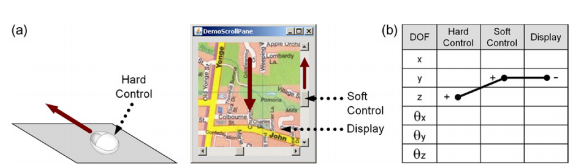
\includegraphics[width=0.7\linewidth]{image/3-6}
		\caption{Source: Figure 3.6 (Mackenzie)}
	\end{figure}
\end{frame}


\begin{frame}
	\frametitle{Rotations}
	\begin{itemize}
		\item Let's consider another possible transformation: \textbf{rotations}
		\item theta ($\theta$) designate angle, whereas positive direction corresponds to clockwise movement
		\item \textbf{Degree of freedom} refers to the degree in which each parameter may be manipulated independently of the others
		\item For a 3D object, six parameters are required: three for the object's position in space (x, y, z), and three for object's orientation in space ($\theta_{x}$, $\theta_{y}$, $\theta_{z}$).  
%		In aeronautics, the rotation terms are known as pitch ($\theta_{x}$), roll ($\theta_{z}$), and $\theta_{y}$.
	\end{itemize}
	\begin{columns}[c]		
		\column{.4\textwidth} % Left column and width
		\begin{figure}
			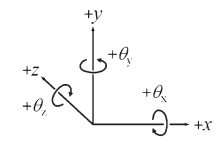
\includegraphics[width=0.6\linewidth]{image/3-7}
			\caption{Source: Figure 3.7 (Mackenzie)}
		\end{figure}
		\column{.4\textwidth} % Right column and width
		\begin{figure}
			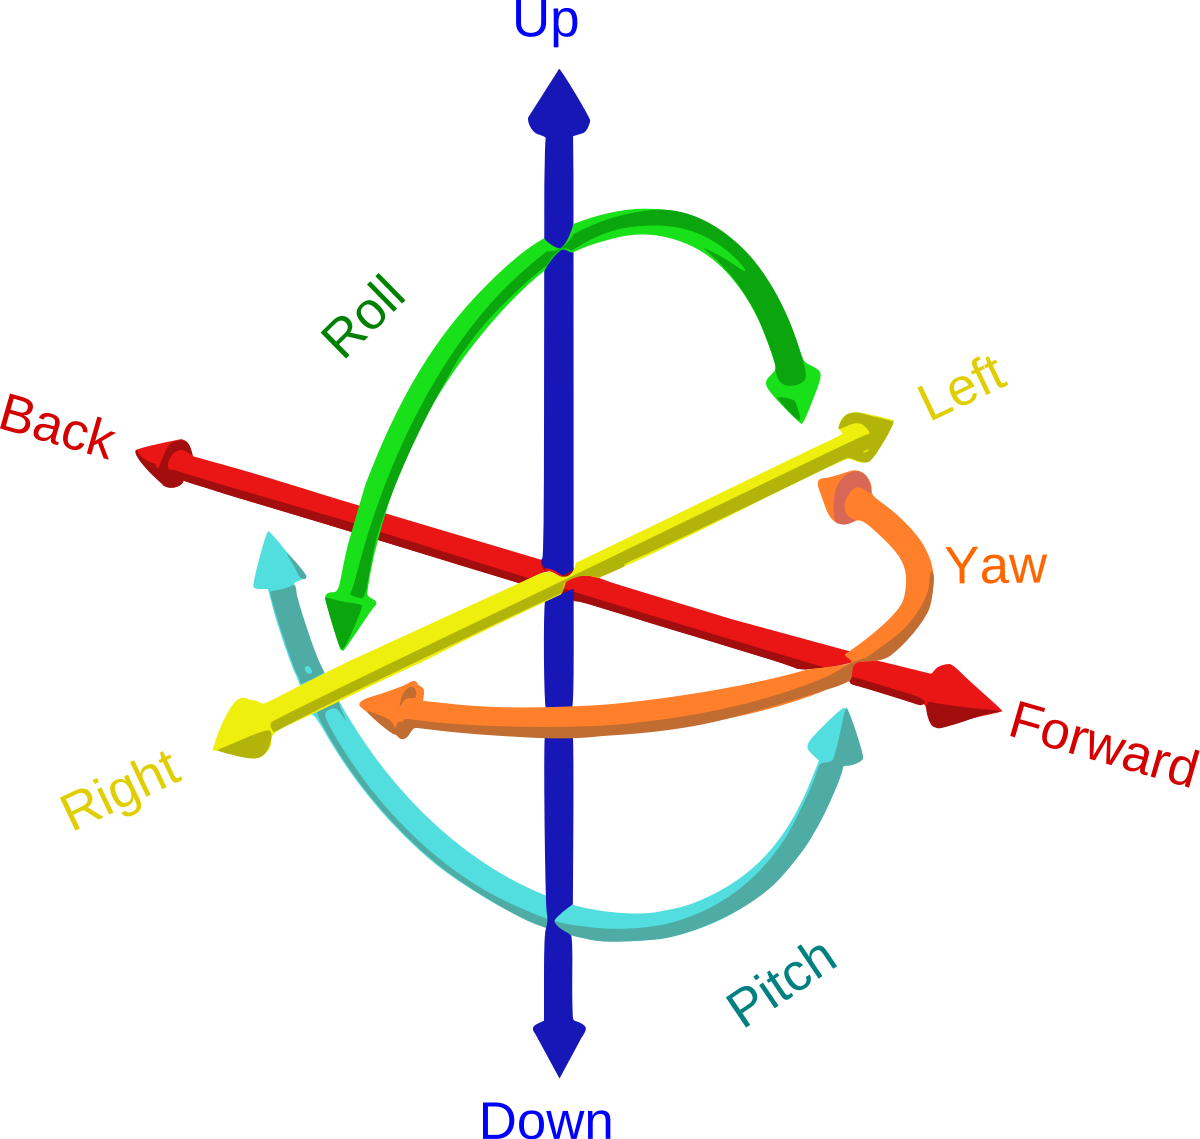
\includegraphics[width=0.4\linewidth]{image/dof}
			\caption{Source: Wikipedia}
		\end{figure}
	\end{columns}

\end{frame}

\begin{frame}
	\frametitle{Rotations}
	An example of exact congruence in 3D space
	\begin{figure}
		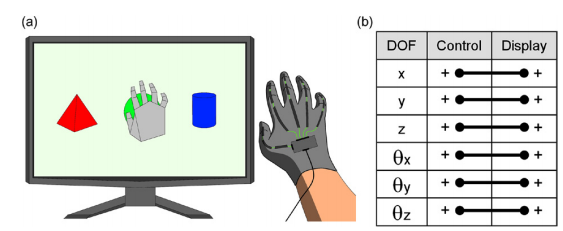
\includegraphics[width=0.7\linewidth]{image/3-8}
		\caption{Source: Figure 3.8 (Mackenzie)}
	\end{figure}
\end{frame}

\begin{frame}
%	\footnotesize
	\frametitle{Rotations}
%	An example of map navigation.
	\begin{itemize}
		\item \textbf{Panning}: drag the mouse where linear movement of the mouse in x-axis (left-right) rotates the display along the y-axis, a linear movement of the z-axis (forward-backward) rotates the scene along the x-axis
		\item \textbf{Zooming}: clicking on + and - soft controls, or use the middle-wheel of a mouse. The middle wheel is a spatially congruent control-display mapping but the problem is its jerkiness (non-continuous).  A better way is to use z-axis movement but oops...%it is already occupied by panning, if then, how to solve?
%		\item A yet unexplored interaction is to use y-axis rotation of the mouse to perform y-axis rotation of the camera to create left-right panning - but why it is not being explored?
	\end{itemize}
	\begin{figure}
		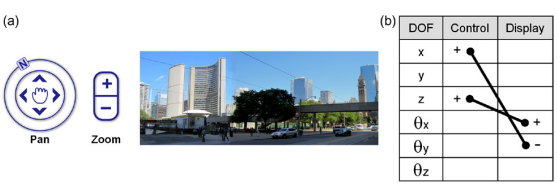
\includegraphics[width=0.5\linewidth]{image/3-9}
		\caption{Source: Figure 3.9 (Mackenzie)}
	\end{figure}
\end{frame}

\subsection{CD gain}

\begin{frame}
	\frametitle{CD gain}
	\begin{itemize}
		\item \textbf{CD gain} refers to the amount of movement in a display object (e.g., cursor), for a given amount of movement in a control. 
		\item For example,   if a mouse is moved three cm,  the cursor moves six cm, then the CD gain is 6/3 = 2
	\end{itemize}
	\begin{figure}
		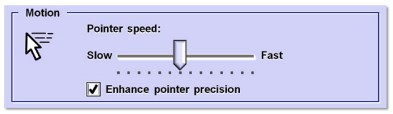
\includegraphics[width=0.7\linewidth]{image/3-10}
		\caption{Source: Figure 3.10 (Mackenzie)}
	\end{figure}
\end{frame}

\begin{frame}
%	\footnotesize
	\frametitle{CD gain}
	\begin{itemize}
%		\item Often, the CD gain relationship is non-linear.  Why?
		\item Follows a \textbf{power function} - enables by "\textit{Enhance pointer precision}".  If the mouse moves quickly, CD gain increases.  Vice versa.
		\item Lowering the CD gain for slow controller movements is useful to enhance the precision of target selection 
		at the end
%		\item The term \textbf{transfer function} is sometimes used. To ensure the cursor is responsive to mouse movement, with no perceivable delay, the software implementation of a non-linear relationship typically uses a \textbf{lookup table} to map controller movement to display movement.
	\end{itemize}
	\begin{figure}
		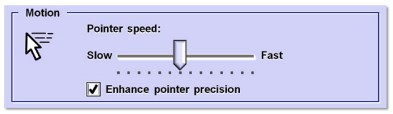
\includegraphics[width=0.7\linewidth]{image/3-10}
		\caption{Source: Figure 3.10 (Mackenzie)}
	\end{figure}
\end{frame}

\begin{frame}
	\frametitle{CD gain}
	\begin{itemize}
		\item Research on CD gain dates back to at least 1940s
		\item Varying CD gain evokes a tradeoff between \textbf{gross positioning time} (getting to the target) and \textbf{fine positioning time} (final acquisition).
%		\item Other confounding factors (e.g., display size or scale) adds to the difficulty of optimization
		\item  CD gain research is still ongoing, although the focus is often in \textbf{different settings} - very large displays, very small displays, remote pointing, accessible computing, 3D interaction

	\end{itemize}
	\begin{figure}
		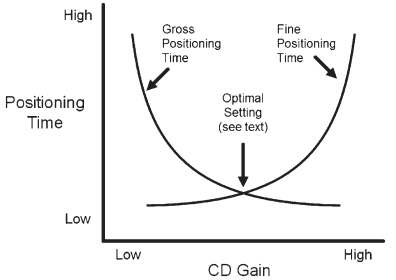
\includegraphics[width=0.35\linewidth]{image/3-11}
		\caption{Source: Figure 3.11 (Mackenzie)}
	\end{figure}
\end{frame}

%\begin{frame}
%	\frametitle{CD gain}
%	\begin{itemize}
%%		\item In the past 30 years, our understanding of CD gain becomes much better.
%%		\item The majority of studies found that significant performance benefits are \textbf{not achieved by adjusting CD gain}
%%		\item One challenge in optimizing CD gain is in defining optimal performance. Is the goal to maximize speed (viz. minimize positioning time) or to maximize accuracy? The goal of optimizing both speed and accuracy is problematic, because of the \textbf{speed-accuracy trade-off}
%	\end{itemize}
%\end{frame}

\subsection{Latency}

\begin{frame}
	\frametitle{Latency}
	\begin{itemize}
		\item Not surprisingly, human performance and the interaction experience are adversely affected when feedback is delayed. The delay between an input action and the corresponding response on a display is called \textbf{latency} or \textbf{lag}.
		\item Latency is crucial in \textbf{remote manipulation} and \textbf{virtual reality}, etc.
%		\item Latency is negligible in many interactive computing tasks, such as typing or cursor positioning but is not true for \textbf{remote manipulation} where huge latency can occur due to transmission delays
%		\item In \textbf{virtual reality} environment, as expected, when lag occurs, the loss of fidelity is dramatic and frustration increases.
	\end{itemize}
\end{frame}

\begin{frame}
	\frametitle{Latency}
	\begin{itemize}
%		\item Latency is attributable to properties of I/O or software.
%		\item Input devices are typically sampled at fixed rates in the range of 10 to 60 samples per second.  At 60Hz sampling, for example, an input movement may not be sensed for 1/60 s = 0.01667s  =  16.67ms.   %Note that latency may increase due to software overhead as well
		\item MacKenzie and Ware (1993) systematically introduced latency in a system and measured the effect on human performance in simple point-select tasks. With \textbf{75ms} latency, movement time increased by 16 percent and \textbf{error rate by 36 percent.} At \textbf{225ms} the effect was dramatic, with movement time increasing by 64 percent and error rate by \textbf{214 percent}
	\end{itemize}
\end{frame}

\subsection{Property sensed}

\begin{frame}
	\frametitle{Property sensed}
	\begin{itemize}
		\item The input controller senses the interaction and coverts a \textbf{property sensed} into data that are transmitted to the host computer for processing. 
		\item For pointing devices, the most common properties sensed are \textbf{position}, \textbf{displacement}, and \textbf{force}. 
		\begin{itemize}
			\item With a \textbf{pen}, the property sensed is the \textbf{position} of a stylus
			\item With \textbf{finger}, the property sensed is the \textbf{absolute coordinate} at the point of contact along the x and z axis
			\item \textbf{Mouse} is different and uses \textbf{displacement} instead which is \textbf{relative} to previous movement.
			\item \textbf{Joystick} also uses \textbf{displacement}
			\item \textbf{Thinkpad trackpoint} uses \textbf{force}
		\end{itemize}
%		\item Another interesting point is to ask whether the property sensed control the position or the velocity of the object or view? This question speaks to the \textbf{order of control}
	\end{itemize}
\end{frame}

%\begin{frame}
%	\frametitle{Property sensed and order of control}
%	\begin{itemize}
%%		\item The most common orders of control are \textbf{position-control} (aka zero-order control) and \textbf{velocity-control} (aka first-order control) (Zhai, 1995, p. 4). With position control, the sensed property of the input device controls the position of the object 
%%		or view on a display. With velocity-control, the sense property controls the velocity of the object or view. A mouse is a position-control input device, since mouse displacement controls the position of the cursor.
%	\end{itemize}
%\end{frame}

\begin{frame}
%	\footnotesize
	\frametitle{Isotonic}
	\begin{itemize}
%		\item Joysticks are either \textbf{isotonic} or \textbf{isometric}.
%		\item With an \textbf{isotonic} joystick, the user manipulates the stick handle, which, in turn, swivels about a pivot-point. The property sensed is the \textbf{movement} of the stick.
		\item Isotonic joysticks are called \textbf{displacement} joysticks. The output signal represents the position of the stick as the amount of displacement (i.e., rotation) from the neutral or home position, about the x- and z-axes.  Good for \textbf{position}.
	\end{itemize}
	\begin{figure}
		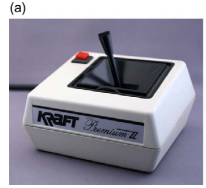
\includegraphics[width=0.4\linewidth]{image/3-13a}
		\caption{Source: Figure 3.13a (Mackenzie)}
	\end{figure}
\end{frame}

\begin{frame}
	\frametitle{Isometric}
	\begin{itemize}
		\item With an \textbf{isometric} joystick, the stick does not move. The property sensed is the \textbf{force} applied to the stick. The output signal represents the amount of force along the x-axis and z-axis. An example is trackpoint build in many Thinkpad laptops.  Good for \textbf{velocity}.
	\end{itemize}
	\begin{figure}
		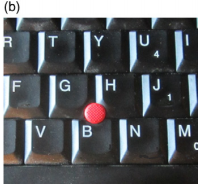
\includegraphics[width=0.35\linewidth]{image/3-13b}
		\caption{Source: Figure 3.13b (Mackenzie)}
	\end{figure}
\end{frame}

%\begin{frame}
%	\frametitle{Isotonic vs. Isometric}
%	\begin{itemize}
%		\item Which mappings are best in terms of speed and accuracy for common point-select tasks?
%		\item Kantowitz and Elvers (1988) evaluated an isometric 
%		joystick in both position-control and velocity-control modes. Velocity-control performed best
%		\item Zhai (1995) observed that position control is best for a position-sensing device 
%		and that velocity control is best for a force-sensing device.
%	\end{itemize}
%	\begin{figure}
%		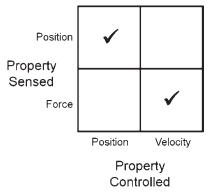
\includegraphics[width=0.3\linewidth]{image/3-14}
%		\caption{Source: Figure 3.14 (Mackenzie)}
%	\end{figure}
%\end{frame}
%
%\begin{frame}
%\begin{center} 
%\usebeamerfont*{frametitle} \usebeamercolor[fg]{frametitle}  5-mins break 
%\end{center}
%\end{frame}

\section{Natural versus learned relationships}

\begin{frame}
	\frametitle{Natural versus learned relationships}
	\begin{itemize}
%		\item It is worth examining which kind of mapping is more natural than others
		\item For the figure below of turning the knob, is it intuitive?
		\item On might argue that clockwise is the same as moving up, thus it is natural.  Nevertheless, this relationship remains a \textbf{"learned"} relationship
	\end{itemize}
	\begin{figure}
		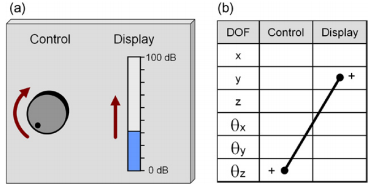
\includegraphics[width=0.7\linewidth]{image/3-15}
		\caption{Source: Figure 3.15 (Mackenzie)}
	\end{figure}
\end{frame}

\begin{frame}
	\frametitle{Natural versus learned relationships}
	\begin{itemize}
		\item Best scenario is spatial congruence, where there is a clear 1-1 mapping.
	\end{itemize}
	\begin{figure}
		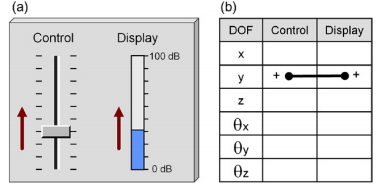
\includegraphics[width=0.7\linewidth]{image/3-16}
		\caption{Source: Figure 3.16 (Mackenzie)}
	\end{figure}
\end{frame}

\begin{frame}
	\frametitle{Natural versus learned relationships}
	\begin{itemize}
		\item Is the switch having a spatial congruence?
		\item Since on/off is not something that has spatial properties, it is difficult to design a spatial congruence
		\item In such case, culture plays a big role.  In UK, a up is off, while in US, the light is on (see how problematic it can be!)
	\end{itemize}
	\begin{figure}
		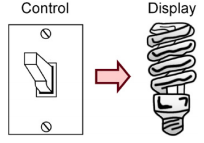
\includegraphics[width=0.4\linewidth]{image/3-17}
		\caption{Source: Figure 3.17 (Mackenzie)}
	\end{figure}
\end{frame}

\begin{frame}
	\frametitle{Natural versus learned relationships}
	\begin{itemize}
		\item Which one is spatially congruent?
	\end{itemize}
	\begin{figure}
		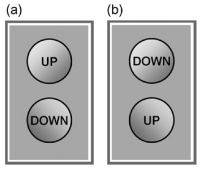
\includegraphics[width=0.4\linewidth]{image/3-18}
		\caption{Source: Figure 3.18 (Mackenzie)}
	\end{figure}
\end{frame}

\section{Metaphor}

\begin{frame}
	\frametitle{Clock as metaphor}
	\begin{itemize}
		\item Most users have a ingrained understanding of a clock
		\item Numerous HCI research use clock as a metaphor to help users do text-entry or to navigate 
	\end{itemize}
	\begin{figure}
		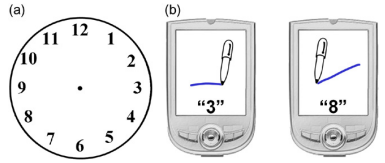
\includegraphics[width=0.7\linewidth]{image/3-20}
		\caption{Source: Figure 3.20 (Mackenzie)}
	\end{figure}
\end{frame}
%
%\begin{frame}
%	\frametitle{Clock as metaphor}
%	\begin{figure}
%		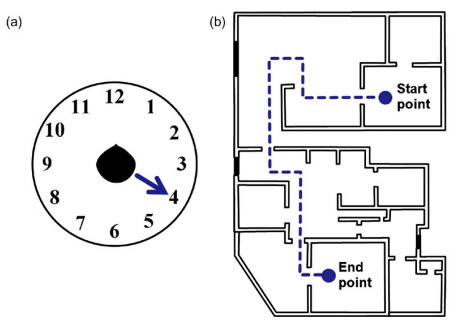
\includegraphics[width=0.7\linewidth]{image/3-21a}
%		\caption{Source: Figure 3.21a (Mackenzie)}
%	\end{figure}
%\end{frame}

\begin{frame}
	\frametitle{Pulse as metaphor}
	\begin{figure}
		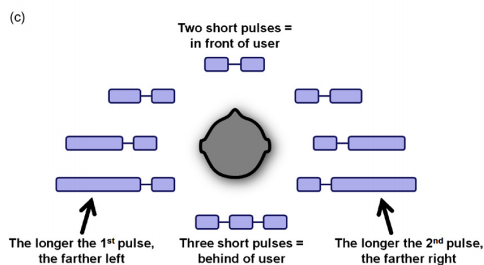
\includegraphics[width=0.9\linewidth]{image/3-21b}
		\caption{Source: Figure 3.21b (Mackenzie)}
	\end{figure}
\end{frame}

\section{Modes}

\begin{frame}
	\frametitle{Modes}
	\begin{itemize}
		\item A common and sometimes frustrating property of user interfaces is \textbf{modes}.
%		\item A mode is the possibilities of a function
		\item Challenges with modes occur because there are \textbf{fewer 
		controls than tasks} %- a standard desktop keyboard has about 100 keys, yet can produce more than 800 key variations, using the modes afforded by modifier keys such as shift, ctrl, alt, function keys.
	\end{itemize}
	\begin{figure}
		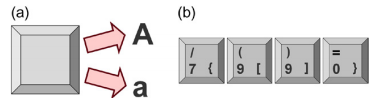
\includegraphics[width=0.9\linewidth]{image/3-22}
		\caption{Source: Figure 3.22 (Mackenzie)}
	\end{figure}
\end{frame}

\begin{frame}
	\frametitle{Modes}
	Modes exist in most interactive systems and are usually difficult to learn
	\begin{figure}
		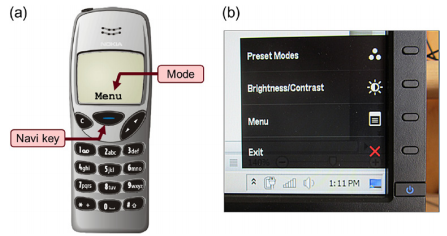
\includegraphics[width=0.9\linewidth]{image/3-23}
		\caption{Source: Figure 3.23 (Mackenzie)}
	\end{figure}
\end{frame}

\begin{frame}
	\frametitle{Modes}
	Changing mode can be easy or difficult!
	\begin{figure}
		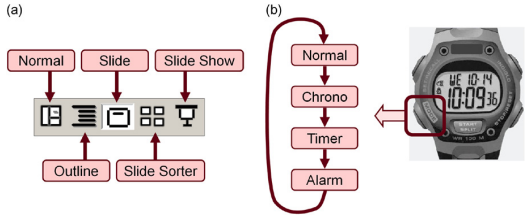
\includegraphics[width=0.9\linewidth]{image/3-24}
		\caption{Source: Figure 3.24 (Mackenzie)}
	\end{figure}
\end{frame}

\begin{frame}
	\frametitle{Modes}
	Feedback is crucial in a mode design system
	\begin{figure}
		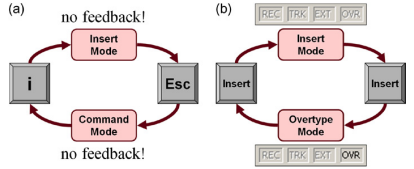
\includegraphics[width=0.9\linewidth]{image/3-25}
		\caption{Source: Figure 3.25 (Mackenzie)}
	\end{figure}
\end{frame}

%\begin{frame}
%	\frametitle{Modes}
%	Modes are common in graphic design software
%	\begin{figure}
%		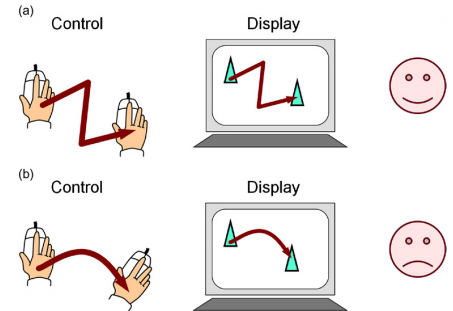
\includegraphics[width=0.7\linewidth]{image/3-26}
%		\caption{Source: Figure 3.26 (Mackenzie)}
%	\end{figure}
%\end{frame}

%\begin{frame}
%	\frametitle{Modes}
%	\begin{itemize}
%		\item I have published a recent paper looking at gesture modes
%		\item Intuitive gestures are limited thus we propose augmenting modifiers
%	\end{itemize}
%	\begin{figure}
%		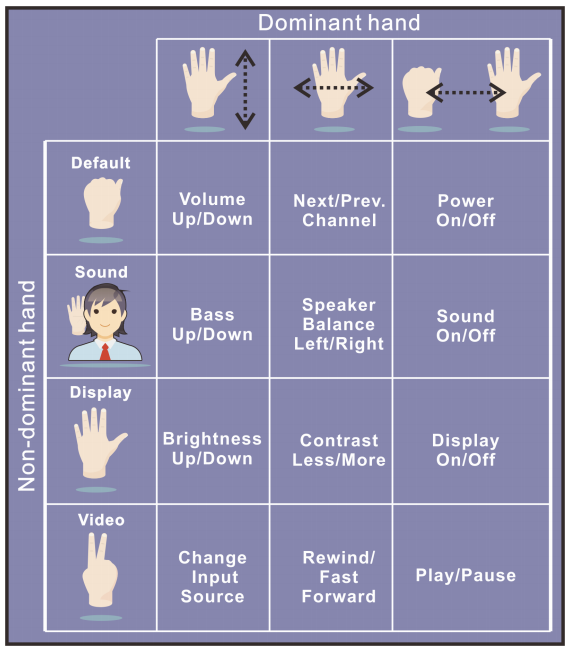
\includegraphics[width=0.4\linewidth]{image/gesture}
%		\caption{Delamare, Silpasuwanchai, Sarcar, Shiraki, Ren (2019)}
%	\end{figure}
%\end{frame}

\section{Bandwidth}

\begin{frame}
	\frametitle{Bandwidth}
	\begin{itemize}
%		\item DOF refers to the interaction bandwidth
		\item Large amount of HCI research focuses on increasing \textbf{interaction bandwidth}%, thus addressing the problem of "hidden" modes
		\item E.g., doctors performing surgery with two hands busy while using eye gestures to perform additional actions
%		\item Current research explores possibilities of new input device as well as augmenting bio-signals
	\end{itemize}
	\begin{figure}
		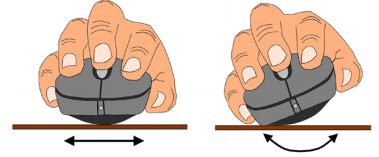
\includegraphics[width=0.7\linewidth]{image/3-31}
		\caption{Source: Figure 3.31 (Mackenzie)}
	\end{figure}
\end{frame}

%\begin{frame}
%	\footnotesize
%	\frametitle{Degrees of freedom}
%	\begin{itemize}
%		\item \textbf{Phantom Premium} offers six degrees of freedom (3 translational, 3 torque) in output capabilities. This device includes a passive stylus and thimble gimbal and provides 3 degrees of freedom positional sensing and 3 degrees of freedom force-feedback. This device can provide force feedback include virtual assembly, virtual prototyping, maintenance path planning, teleoperation, and molecular modeling.
%	\end{itemize}
%	\begin{figure}
%		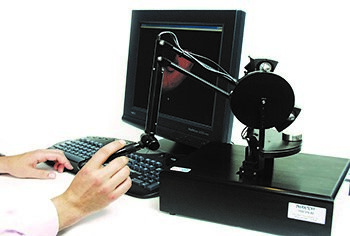
\includegraphics[width=0.5\linewidth]{image/phantom}
%		\caption{Phantom Premium 1.4}
%	\end{figure}
%\end{frame}

\begin{frame}
%	\footnotesize
	\frametitle{Bandwidth}
	\begin{itemize}
		\item Click anywhere you want
	\end{itemize}
	\begin{figure}
		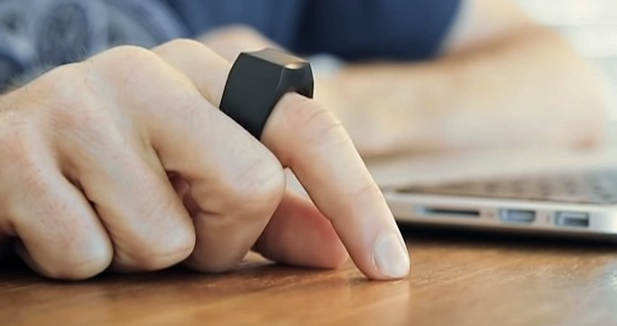
\includegraphics[width=0.7\linewidth]{image/ringmouse}
		\caption{EasySMX Ring: provides convenience but loses full-featured mouse when it comes to productivity}
	\end{figure}
\end{frame}

\begin{frame}
%	\footnotesize
	\frametitle{Bandwidth}
	\begin{itemize}
		\item Chair gestures
	\end{itemize}
	\begin{figure}
		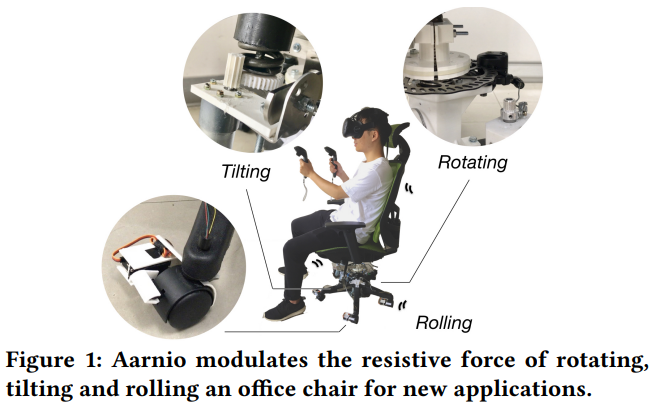
\includegraphics[width=0.7\linewidth]{image/chairgestures}
		\caption{Teng et al., \textbf{Aarnio: Passive Kinesthetic Force Output for Foreground Interactions on an Interactive Chair}, CHI 2019}
	\end{figure}
\end{frame}

\begin{frame}
	\frametitle{Activities}
	\begin{block}{Classwork}
		\footnotesize
		\begin{itemize}
			\item Download \textbf{GoFitts.jar} from \url{http://www.yorku.ca/mack/FittsLawSoftware/}
			\item Perform a 1D fitts tasks with default settings (\textbf{A} = 100, 200, 400; \textbf{W} = 20, 40, 80).  Other factors include \textbf{pointing speed} - \textit{slow, medium, fast}, and \textbf{precision mode} - \textit{on \& off}.    If you are NOT using Windows, instead of precision mode, use \textbf{handedness} instead (left and right hand).    Set the \textbf{Number of Trials} to 5.  Set \textbf{Condition Code} according to the point speed and precision mode.  Leave Session Code and Group Code as default.
			\item Perform\textbf{ four-way ANOVA} with pointing speed, precision mode, A, and W as IV and MT as DV.   (you may want to first convert the long table format to wide format).  
			\item Summarize your result in APA with graphs and submit to GC.
		\end{itemize}
	\end{block}
\end{frame}

%\section{What's next}

\begin{frame}
\frametitle{What's next}
Read slide on \textbf{Modeling}.
\begin{itemize}
	\item Mackenzie, Chapter 7, \textbf{Modeling Interaction},  Human Computer Interaction: An Empirical Research Perspective, 1st ed. (2013) 
\end{itemize}
We will reuse this Fitts data for further modeling.
\end{frame}

%\begin{frame}
%\frametitle{Activities}
%\begin{block}{Classwork}
%	Perform the classwork on Menu Design.  This task requires you to investigate why designing menu is such a difficult task for designers.
%\end{block}
%\end{frame}

\begin{frame}
\Huge{\centerline{Questions}}
\end{frame}

%----------------------------------------------------------------------------------------

\end{document} 
